%
% 3-buch.tex
%
% (c) 2025 Prof Dr Andreas Müller
%
\section{Zu diesem Buch}
\kopfrechts{Zu diesem Buch}
In diesem Buch wird daher zunächst die Idee des Feldes am 
Beispiel des Temperaturfeldes in Kapitel~\ref{chapter:fallstudie}
genauer untersucht.
Dabei wird herausgearbeitet, für welche physikalischen Konzepte
mathematische Abstraktionen entwickelt werden müssen.
Ein zentrale Erkenntnis wird sein, dass das Koordinatensystem keine
Rolle spielen darf.
Um diesem Umstand Rechnung zu tragen, muss es möglich sein, die
Feldgleichungen vollständig unabhängig vom Koordinatensystem
zu formulieren.
Koordinatensysteme werden zwar zur Berechnung eines Feldes immer
noch nötig sein, aber es soll einen klar vorgezeichneten Prozess
geben, wie man aus den koordinatenunabhängig definierten Feldgleichungen
zu einer Koordinatengleichung kommen kann, die dann mit geeigneter
Numeriksoftware gelöst werden kann.
Kapitel~\ref{chapter:koordinaten} entwickelt die Begriffe der
Mannigfaltigkeit, eines Koordinatensystems für eine Mannigfaltigkeit,
der Tangentialvektoren und der Ableitung in einem koordinatenfreien
Kontext.

Kurven auf einer Mannigfaltigkeit und ihre Tangentialvektoren 
beschreiben die Bewegung von Teilchen.
Man kann sich darunter den Experimentator vorstellen, der sich
im Universunm von Punkt zu Punkt bewegt und Messungen vornimmt.
Er versucht, einen Zusammenhang zwischen seinen Beobachtungen
und seiner Bewegung herzustellen.
In Kapitel~\ref{chapter:kurvenintegral} wird untersucht, wie man
physikalische Grössen modelliert, die von der Bewegungsrichtung
und -gschwindigkeit des Experimentators abhängen.
Es entwickelt den Begriff der 1-Formen, der Kurvenintegrale und
des Gradienten einer Funktion.
\index{1-Form}%
\index{Gradient}%

Gewisse physikalische Grössen werden gemessen, indem man Beobachtungen
entlang einer berandeten Fläche durchführt.
Dies führt auf den Begriff der 2-Vektoren, 2-Formen und der Integration
über eine Fläche.
\index{2-Vektor}%
\index{2-Form}%
\index{Integration}
Dies wird in Kapitel~\ref{chapter:green} studiert.
Es werden sich dabei auch der Satz von Green und der Satz von Stokes
ergeben.
Die äussere Ableitung wird als ein koordinatenunabhängiger
Differentialoperator erkannt, die Feldgleichungen für solche
Messgrössen liefern kann.

Die Ideen der 1- und 2-Formen können für beliebige Dimensionen
weiterentwickelt werden.
In Kapitel~\ref{chapter:gauss} wird die Idee der Divergenz eines
Vektorfeldes in einem $n-1$-dimensionalen Raum entwickelt und der
Satz von Gauss bewiesen.
Sie ergibt sich als der Differentialoperator der äusseren Ableitung
auf $n-1$-Formen.
Physikalische Erhaltungssätze werden durch eine Kontinuitätsgleichung
\index{Erhaltungssatz}%
dargestellt, die die Divergenz verwendet.
\index{Divergenz}%

Auch für alle Dimensionen $p$ zwischen $2$ und $n-1$ können $p$-Formen und
eine äussere Ableitung definiert werden, so dass nötigenfalls 
in jeder beliebigen Dimension koordinatenunabhängig definierte
Operatoren zur Verfügung stehen (Kapitel~\ref{chapter:pformen}).
Auf einer Mannigfaltigkeit mit einer Metrik kann aber noch ein weiterer
Operator definiert werden.
Dieser sogenannte Hodge-Operator ist ebenfalls Koordinatenunabhängig
definierbar und kann mit der äusseren Ableitung beliebig kombiniert
werden.
\index{Hodge-Operator}%
Tatsächlich wird in Kapitel~\ref{chapter:hodge} gezeigt, dass alle
Differentialoperatoren der klassischen Vektoranalysis durch Verknüpfung
von äusserer Ableitung und Hodge-Operator entstehen.
Insbesondere gehört dazu auch der Laplace-Operator, der in fast
\index{Laplace-Operator}%
jeder Feldgleichung zweiter Ordnung der Physik vorkommt.

Eine Übersicht über wichtige Feldgleichungen der Physik wird
in Kapitel~\ref{chapter:feldgleichungen} gegeben.
Die Numerik der partiellen Differentialgleichungen ist ein sehr
weitschweifiges Gebiet, in dem auch viel aktive Forschung stattfindet.
Einen Einblick in ein paar wenige Grundideen gibt das
Kapitel~\ref{chapter:pdenumerik}.

Die äussere Ableitung leitet skalare Funktionen oder $p$-Formen
mit skalaren Werten ab.
In der klassischen Vektoranalysis werden Operatoren konstruiert,
mit denen sich ein Vektorfeld ableiten lässt.
Die Entwicklung in den Kapiteln \ref{chapter:green}--\ref{chapter:hodge}
hat aber gezeigt, dass sich diese Operatoren alle durch die
vereinheitlichte Theorie der $p$-Formen und der äusseren Ableitung
formulieren lässt.
Bei der Beschreibung einer Strömung funktioniert das nicht mehr.
Die Strömung transportiert Eigenschaften der Strömung mit sich,
die sowohl skalaren wie auch vektoriellen Charakter haben.
Die Veränderung des Geschwindigkeitsvektors in einem Punkt hängt
nicht nur von den auf die Strömung wirkenden Kräften ab, sondern
rührt auch daher, dass der Impuls des vorbeifliessenden Fluids
örtlich variert.
Auch beim Paralleltransport eines Vektors auf einer gekrümmten
\index{Paralleltransport}%
Oberfläche sind die Tangentialebenen in verschiedenen Punkten nicht
notwendigerweise parallel und es ist somit nicht klar, wie
Tangentialvektoren in nahe beeinander liegenden Punkten überhaupt
miteinander verglichen werden können.
Ein neues mathematisches Konstrukt, ein sogenannter Zusammenhang
\index{Zusammenhang}%
und die daraus konstruierte kovariante Ableitung ist dafür nötig
(Kapitel~\ref{chapter:zusammenhang}).
Die kovariante Ableitung tritt in den Strömungsdifferentialgleichungen
\index{Ableitung!kovariant}%
\index{kovariante Ableitung}%
wie auch in den Differentialgleichungen für Geodäten auf.
\index{Geodate@Geodäte}%

Der Paralleltransport eines Vektors entlang dem Rand eines
geschlossenen Weges kann verraten, ob eine Fläche gekrümmt ist, 
dies in Abbildung~\ref{buch:einleitung:fig:kruemmung} gezeigt ist.
%
% fig-kruemmung.tex
%
% (c) 2025 Prof Dr Andreas Müller
%
\begin{figure}
\centering
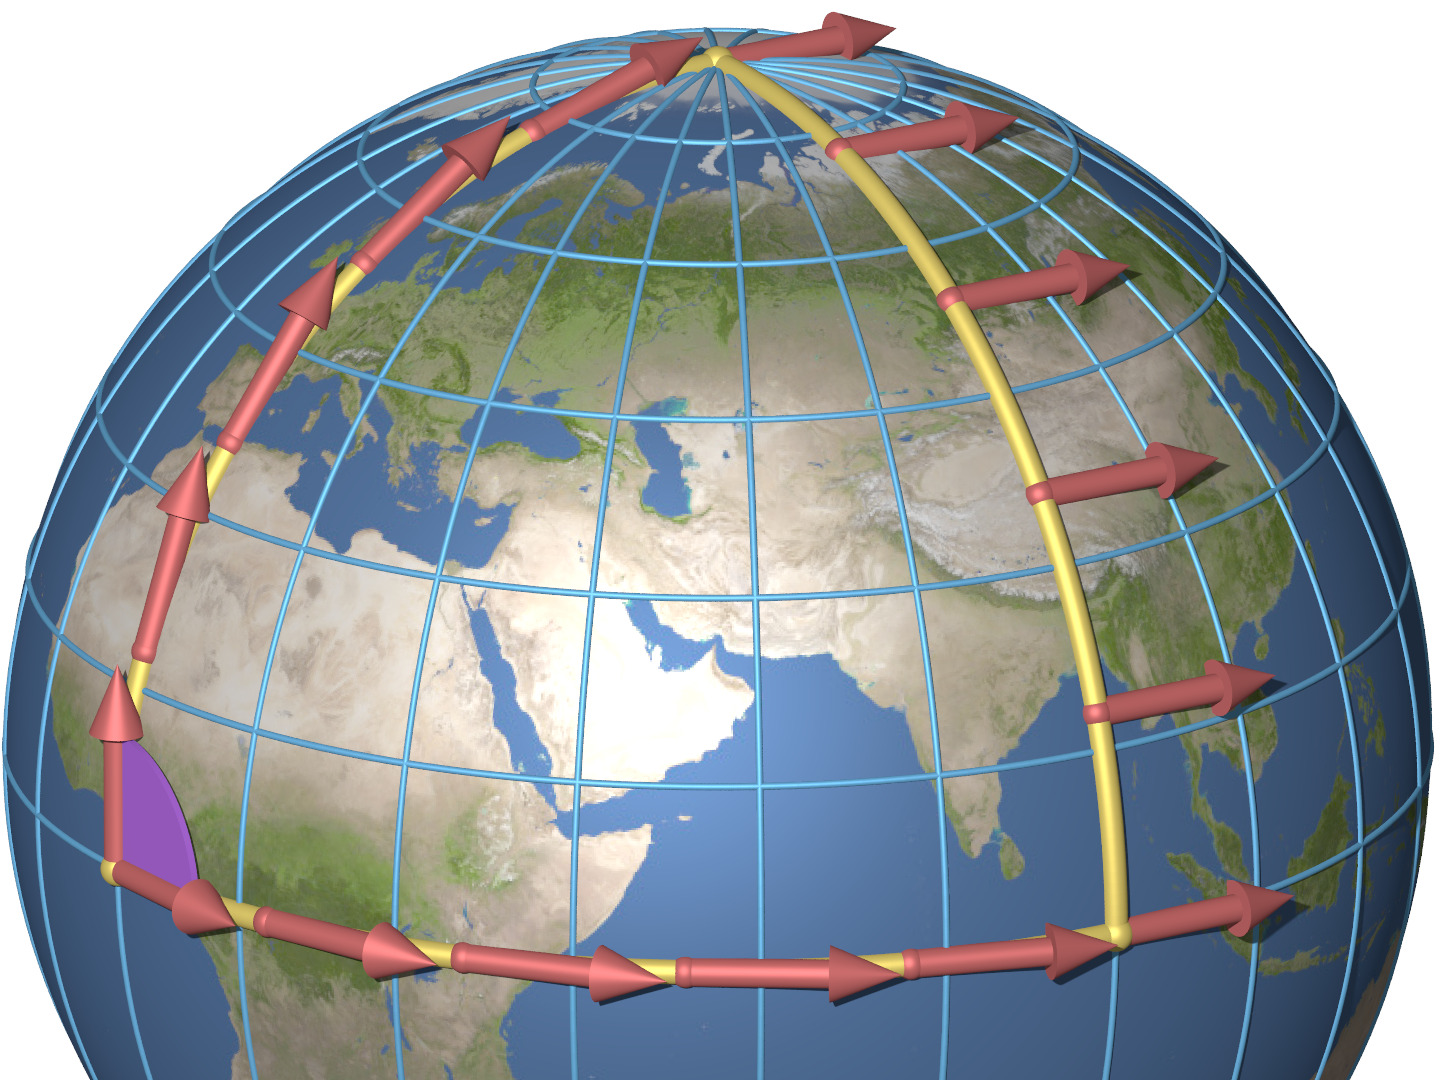
\includegraphics[width=9cm]{chapters/000-einleitung/images/kruemmung.jpg}
\caption{Der Paralleltransport des roten Vektors zunächst entlang des
Äquators, dann entlang eines Längenkreises zum Nordpol und schliesslich
entlang eines weiteren Längenkreises zurück zum Ausgangspunkt führt zu
einer von der Krümmung der Kugeloberfläche verursachten Drehung des
Vektors um den violetten $90^\circ$-Winkel.
\label{buch:einleitung:fig:kruemmung}}
\end{figure}
%
Der riemannsche Krümmungstensor formalisiert diese Idee und wird
\index{Krummungstensor@Krümmungstensor}%
in Kapitel~\ref{chapter:kruemmung} eingeführt.
Albert Einstein hat erkannt, dass sich die Wirkung der Gravitation
\index{Einstein, Albert}%
darin äussert, dass Tangentialvektoren beim Paralleltransport 
ihre Richtung ändern.
Er hat dann eine Gleichung gefunden, die die Krümmung mit dem
Energie- und Impulsgehalt des Raumes verknüpft.
Die allgemeine Relativitätstheorie hat erstmals ermöglicht,
\index{allgemeine Relativitatstheorie@allgemeine Relativitätstheorie}%
\index{Relativitatstheorie, allgemein@Relativitätstheorie, allgemein}%
objektive Aussagen über die langfristige Entwicklung des
Universums zu machen.

Differentialoperatoren analysieren eine physikalische Situation
rein lokal.
Es scheint auf den ersten Blick undenkbar, dass sich daraus globale
Aussagen zum Beispiel über das Strömungsfeld der Erdatmosphäre oder
über das Universum ableiten lassen.
Ein erster Hinweis darauf, dass dies nicht unbedingt zutrifft, sind
die Voraussetzungen des Poincaré-Lemmas von Kapitel~\ref{chapter:pformen}:
\index{Poincare-Lemma@Poincaré-Lemma}%
Es gilt nur auf sternförmigen oder zusammenziebaren Gebieten.
Wenn das Poincaré-Lemma auf einem Gebiet nicht zutrifft, lässt sich
daraus ableiten, dass das Gebiet nicht zusammenziebar sein kann.
Die de~Rham-Kohomologie-Theorie führt diese Idee konsequent zu einer
\index{Kohomologie, de Rham-}%
Analyse der grossräumigen Eigenschaften einer Mannigfaltigkeit.
Sie produziert Invarianten, mit denen sich zum Beispiel eine Kugel
oder ein Torus zuverlässig unterscheiden lassen.
Im Umkehrschluss zeigt sie auch, dass die Topologie einen Einfluss
\index{Topologie}%
auf die möglichen Lösungen einer Feldgleichung haben müssen.
Diese Eigenschaften gelten sogar schon für gewöhnliche
Differentialgleichugen.
Die Morse-Theorie zeigt, wie sich aus den Eigenschaften der Nullstellen
\index{Morse-Theorie}%
eines Vektorfeldes die Gestalt einer Mannigfaltigkeit ablesen lässt.
Kapitel~\ref{chapter:topologie} gibt eine Einführung in diese 
Ideenwelt.

Im zweiten Teil des Buches werden einzelne Themen individuell
vertieft oder angewendet.
Ein Übersicht der Arbeiten wird zu Beginn auf Seite~\pageref{buch:uebersicht}
gegeben.

